\section{From Tests to Transformers}\label{sec:transformer}

The BLB test binaries are not standalone benchmarks --- each exercises a specific cryptographic primitive that corresponds to a layer in private Transformer inference.
This section explains how the test suite maps onto the Transformer architectures evaluated in the BLB paper~\cite{xu2025breaking} (BERT-base, BERT-large, and GPT2-base) and contextualises our unit-test measurements against the paper's end-to-end results.

\paragraph{Important distinction.}
Our test binaries (\texttt{test\_ntt}, \texttt{test\_matmul}, etc.) are \emph{unit tests} for individual cryptographic primitives.
The paper's end-to-end inference is driven by a single binary (\texttt{ckks\_bert\_large\_main}) that chains all primitives, applies FineGrainFusion, and manages the CKKS\,/\,MPC transitions across layers.
The numbers in Section~\ref{ssec:paper-results} come from the paper; Section~\ref{ssec:test-mapping} maps our unit tests onto the operations inside that pipeline.

%% ---------------------------------------------------------------
\subsection{Private Transformer Inference Pipeline}

A Transformer block (as in BERT or GPT-2~\cite{xu2025breaking}) consists of:
\begin{enumerate}[nosep]
  \item \textbf{Multi-Head Self-Attention}: $Q, K, V$ projections (linear), attention scores ($QK^T / \sqrt{d_h}$), softmax, weighted sum, output projection (linear).
  \item \textbf{Layer Normalization}: mean, variance, normalise, affine transform.
  \item \textbf{Feed-Forward Network (FFN)}: linear $\to$ GeLU $\to$ linear.
  \item \textbf{Layer Normalization} (again).
\end{enumerate}

\paragraph{Ring parameters (\S7.1 of the paper).}
BLB operates over the ring $\mathbb{Z}_Q[X]/(X^N+1)$ with
ring-element bitwidth $\ell = 43$~bits,
fixed-point scale $s = 13$,
and computational security parameter $\lambda = 128$.
The CKKS polynomial degree is $N = 2^{13} = 8192$, yielding $N/2 = 4096$ usable slots per ciphertext.

\paragraph{Hybrid CKKS\,+\,MPC design.}
In BLB's model each operation is assigned to the most efficient backend:
\textbf{linear layers use HE} (CKKS ciphertext rotations on packed polynomials, no communication rounds beyond the initial encoding) while
\textbf{nonlinear operations use MPC} (OT-based comparison requires communication but avoids expensive HE bootstrapping).
This hybrid approach breaks the ``layer barrier'' --- previous systems required HE bootstrapping or MPC round-trips for every layer, but BLB keeps data in the HE domain across multiple consecutive linear layers, switching to MPC only for nonlinearities.

\paragraph{FineGrainFusion (Figure~10 in the paper).}
After applying FineGrainFusion, a single Transformer block is decomposed into \textbf{five fused blocks} of linear operators.
Each fused block chains several weight matrices (e.g.\ $W_Q$, $W_K$, $W_V$ of the same head) into a single CKKS MatMul call, amortising rotation costs and eliminating intermediate HE-to-MPC transitions.
MPC evaluation is inserted only at the boundaries between fused blocks, where a nonlinear function (softmax, GeLU, or LayerNorm) is required.

%% ---------------------------------------------------------------
\subsection{Models Evaluated in the Paper}\label{ssec:models}

The paper evaluates three Transformer architectures.
Note the inclusion of GPT2-base, which demonstrates that BLB generalises beyond BERT encoder models to autoregressive decoders.

\begin{table}[ht]
\centering
\caption{Transformer models evaluated in BLB~\cite{xu2025breaking}}
\label{tab:model-variants}
\begin{tabular}{lrrrrr}
\toprule
\textbf{Model} & \textbf{Layers} ($L$) & \textbf{Hidden} ($H$) & \textbf{Heads} ($A$) & \textbf{Seq.\ len} ($s$) & \textbf{Params} \\
\midrule
GPT2-base   & 12 & 768  & 12 & 64  & 117\,M \\
BERT-base   & 12 & 768  & 12 & 128 & 110\,M \\
BERT-large  & 24 & 1024 & 16 & 128 & 340\,M \\
\bottomrule
\end{tabular}
\end{table}

{\small Head dimension $d_h = H/A$: 64 for all three models.
FFN intermediate dimension $H_{\text{FFN}} = 4H$: 3072 (base) and 4096 (large).}

%% ---------------------------------------------------------------
\subsection{End-to-End Results from the Paper}\label{ssec:paper-results}

Table~\ref{tab:e2e-results} reproduces the key results from the paper's Table~9.
All numbers are for \textbf{LAN} (0.02\,ms RTT, 5\,Gbps) two-party inference.
The paper's testbed uses a 2.7\,GHz Intel Xeon Platinum 8558P with 64 threads and an NVIDIA A100 GPU --- significantly more powerful than our reproduction testbed (dual Xeon Silver 4208, 32 threads, no GPU; see Section~\ref{sec:evaluation}).

\begin{table}[ht]
\centering
\caption{End-to-end private Transformer inference: BLB vs.\ prior work (LAN, Table~9 of~\cite{xu2025breaking})}
\label{tab:e2e-results}
\begin{tabular}{ll rrr}
\toprule
\textbf{Model} & \textbf{Framework} & \textbf{CPU (min)} & \textbf{GPU (min)} & \textbf{Comm.\ (GB)} \\
\midrule
\multirow{4}{*}{BERT-base}
  & Iron~\cite{iron2022}        & 66.7  & ---   & ---   \\
  & BOLT~\cite{pang2024bolt}        & 22.1  & ---   & 63.6  \\
  & Bumblebee~\cite{lu2023bumblebee} & 5.0 & ---   & 5.8   \\
  & \textbf{BLB}            & \textbf{6.1} & \textbf{2.5} & \textbf{3.0} \\
\midrule
\multirow{4}{*}{BERT-large}
  & Iron~\cite{iron2022}        & 92.0  & ---   & ---   \\
  & BOLT~\cite{pang2024bolt}        & 57.6  & ---   & 158.9 \\
  & Bumblebee~\cite{lu2023bumblebee} & 10.6 & --- & 15.2  \\
  & \textbf{BLB}            & \textbf{15.1} & \textbf{6.6} & \textbf{7.8} \\
\midrule
GPT2-base
  & \textbf{BLB}            & \textbf{4.0}  & \textbf{2.0} & \textbf{1.5} \\
\bottomrule
\end{tabular}
\end{table}

\paragraph{Key improvements.}
\begin{itemize}[nosep]
  \item \textbf{Communication}: BLB achieves a $\mathbf{21\times}$ reduction in communication vs.\ BOLT (e.g.\ 3.0\,GB vs.\ 63.6\,GB for BERT-base) and $\sim\!2\times$ vs.\ Bumblebee (3.0\,GB vs.\ 5.8\,GB).
  \item \textbf{Latency (GPU)}: BLB with GPU acceleration achieves $\sim\!\mathbf{13\times}$ speedup over BOLT and $\sim\!1.8\times$ over Bumblebee on BERT-large (6.6\,min vs.\ 57.6\,min and 10.6\,min respectively, comparing BLB GPU to prior CPU).
  \item \textbf{Communication is the bottleneck}: Even on CPU, BLB's latency is comparable to Bumblebee (6.1\,min vs.\ 5.0\,min for BERT-base). The dominant advantage is the dramatic reduction in communication, which is critical for WAN deployment and scaling to larger models.
\end{itemize}

\paragraph{Hardware gap with our testbed.}
The paper's Xeon Platinum 8558P (2.7\,GHz, 64 threads, A100 GPU) is roughly $2{-}3\times$ more powerful than our Xeon Silver 4208 (2.1\,GHz, 32 threads, no GPU).
Our unit-test measurements on individual primitives should therefore be interpreted as \emph{upper bounds} relative to what the paper's hardware would achieve on the same operations.

%% ---------------------------------------------------------------
\subsection{Scaling Chart}\label{ssec:scaling-chart}

\begin{figure}[ht]
\centering
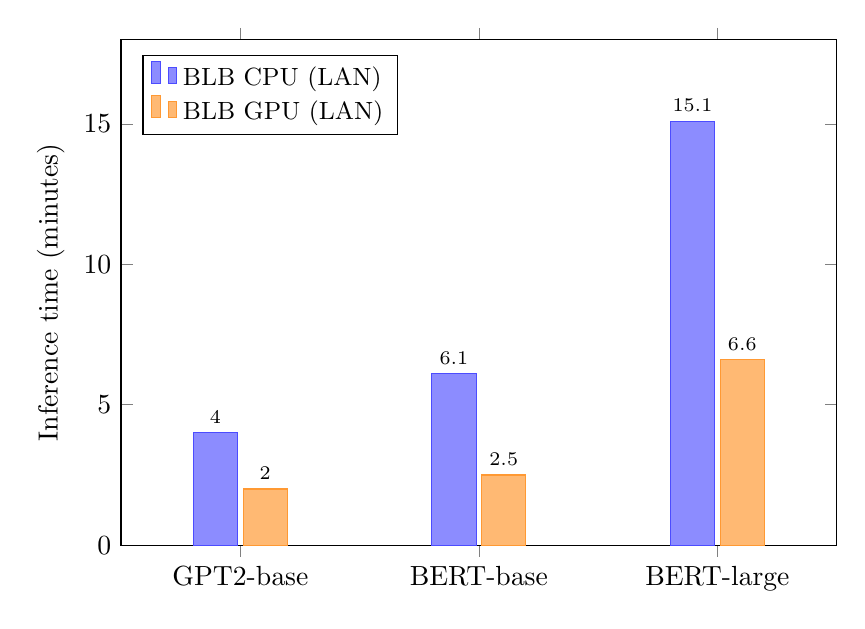
\begin{tikzpicture}
\begin{axis}[
    ybar,
    width=0.88\textwidth,
    height=8cm,
    ylabel={Inference time (minutes)},
    symbolic x coords={GPT2-base, BERT-base, BERT-large},
    xtick=data,
    ymin=0, ymax=18,
    bar width=16pt,
    nodes near coords,
    every node near coord/.append style={font=\scriptsize, rotate=0},
    enlarge x limits=0.25,
    legend style={at={(0.03,0.97)}, anchor=north west, font=\small},
    legend cell align={left},
]
\addplot[fill=blue!45, draw=blue!70] coordinates {
    (GPT2-base, 4.0)
    (BERT-base, 6.1)
    (BERT-large, 15.1)
};
\addlegendentry{BLB CPU (LAN)}

\addplot[fill=orange!55, draw=orange!80] coordinates {
    (GPT2-base, 2.0)
    (BERT-base, 2.5)
    (BERT-large, 6.6)
};
\addlegendentry{BLB GPU (LAN)}
\end{axis}
\end{tikzpicture}
\caption{BLB end-to-end private inference times from the paper's Table~9 (LAN setting). GPU acceleration via PhantomFHE reduces latency by $1.6{-}2.4\times$ across models. The sub-linear scaling from BERT-base to BERT-large (2.5$\times$ on CPU despite $2\times$ layers and $1.33\times$ hidden dim) reflects the effectiveness of FineGrainFusion.}
\label{fig:scaling}
\end{figure}

\begin{figure}[ht]
\centering
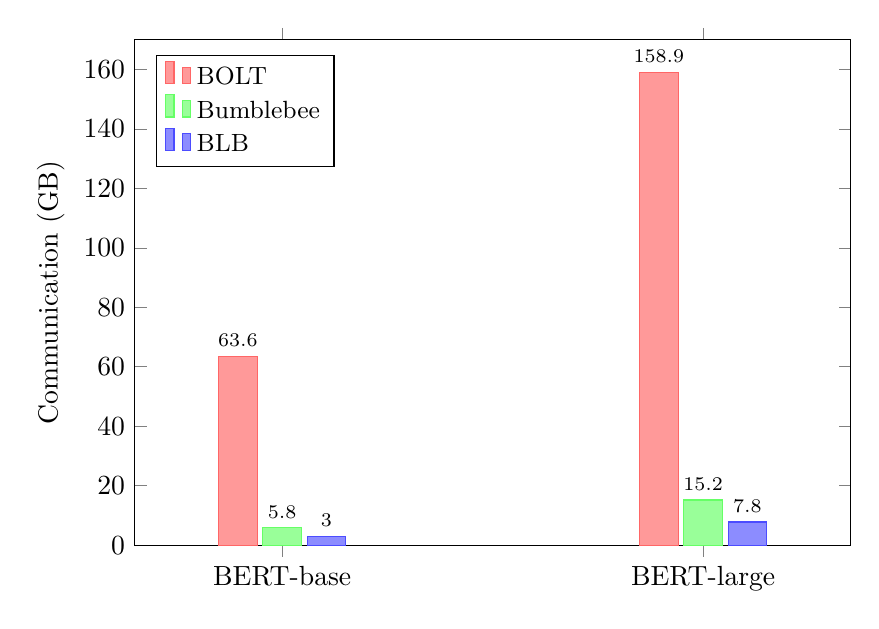
\begin{tikzpicture}
\begin{axis}[
    ybar,
    width=0.88\textwidth,
    height=8cm,
    ylabel={Communication (GB)},
    symbolic x coords={BERT-base, BERT-large},
    xtick=data,
    ymin=0, ymax=170,
    bar width=14pt,
    nodes near coords,
    every node near coord/.append style={font=\scriptsize},
    enlarge x limits=0.35,
    legend style={at={(0.03,0.97)}, anchor=north west, font=\small},
    legend cell align={left},
]
\addplot[fill=red!40, draw=red!60] coordinates {
    (BERT-base, 63.6)
    (BERT-large, 158.9)
};
\addlegendentry{BOLT}

\addplot[fill=green!40, draw=green!60] coordinates {
    (BERT-base, 5.8)
    (BERT-large, 15.2)
};
\addlegendentry{Bumblebee}

\addplot[fill=blue!45, draw=blue!70] coordinates {
    (BERT-base, 3.0)
    (BERT-large, 7.8)
};
\addlegendentry{BLB}
\end{axis}
\end{tikzpicture}
\caption{Communication cost comparison (LAN). BLB achieves $21\times$ reduction vs.\ BOLT and $\sim\!2\times$ vs.\ Bumblebee. The communication gap widens with model size: BLB's 7.8\,GB for BERT-large is 20$\times$ less than BOLT's 158.9\,GB.}
\label{fig:comm-comparison}
\end{figure}

%% ---------------------------------------------------------------
\subsection{Test-to-Operation Mapping}\label{ssec:test-mapping}

Table~\ref{tab:transformer-mapping} maps each of our unit-test binaries to the Transformer operations it exercises.
These tests validate individual primitives; the paper's end-to-end pipeline fuses multiple primitives via FineGrainFusion and uses the CKKS MatMul protocols (not circulant linear alone) as the primary linear-layer mechanism.

\begin{table}[ht]
\centering
\caption{Mapping Transformer operations to BLB cryptographic primitives and our test binaries}
\label{tab:transformer-mapping}
\begin{tabular}{p{4cm}p{3.5cm}p{2.5cm}p{3cm}}
\toprule
\textbf{Transformer Op} & \textbf{BLB Primitive} & \textbf{Backend} & \textbf{Test Binary} \\
\midrule
$Q, K, V$ projections        & CKKS MatMul / CirLinear & HE (CKKS)   & \texttt{test\_cir\_linear} \\
Attention $QK^T$              & CKKS MatMul (diagonal)  & HE (CKKS)   & \texttt{test\_matmul} \\
Attention softmax             & FixPoint comparison      & MPC (OT)    & \texttt{test\_fixpoint} \\
Attention $\text{softmax} \cdot V$ & CKKS MatMul (diagonal) & HE (CKKS) & \texttt{test\_matmul} \\
Attention output projection   & CKKS MatMul / CirLinear & HE (CKKS)   & \texttt{test\_cir\_linear} \\
LayerNorm (mean, var, scale)  & FixPoint truncate/round  & MPC (OT)    & \texttt{test\_fixpoint} \\
FFN first linear              & CKKS MatMul / CirLinear & HE (CKKS)   & \texttt{test\_cir\_linear} \\
FFN activation (GeLU)         & Piecewise poly + MPC     & HE+MPC      & \texttt{test\_linear\_operator} \\
FFN second linear             & CKKS MatMul / CirLinear & HE (CKKS)   & \texttt{test\_cir\_linear} \\
\bottomrule
\end{tabular}
\end{table}

%% ---------------------------------------------------------------
\subsection{Primitive Details}

\subsubsection{test\_ntt: Polynomial Foundation}

Every CKKS operation ultimately reduces to NTT (Number Theoretic Transform) on polynomials in the ring $\mathbb{Z}_Q[X]/(X^N+1)$.
When SEAL evaluates a ciphertext rotation or multiplication, it performs forward NTT, element-wise multiply in the NTT domain, and inverse NTT.
Intel HEXL accelerates this with AVX-512 SIMD intrinsics.

\textbf{Role in Transformer}: \texttt{test\_ntt} validates the foundation that \emph{every other HE operation} builds on.
A single BERT-base layer with $H{=}768$ involves hundreds of NTT operations for the rotation-based matrix multiplication within each of the five fused blocks.

\subsubsection{test\_linear\_operator: HE Element-Wise Computation}

Tests CKKS element-wise operations: $\mathbf{x}^2$ and $\mathbf{x} \odot \mathbf{y}$ on 8192-slot ciphertexts with values in $[-5, 5]$.

\textbf{Role in Transformer}: Element-wise multiply is the primitive for:
\begin{itemize}[nosep]
  \item \textbf{GeLU activation}: BLB adopts BOLT's piecewise polynomial approximation with Motzkin preprocessing:
  \[
  \text{ApproxGeLU}(x) = \begin{cases}
    x & \text{if } x > 2.7, \\
    0 & \text{if } x < -2.7, \\
    g_0 + g_1 x + g_2 x^2 + g_3 x^3 + g_4 x^4 & \text{otherwise},
  \end{cases}
  \]
  with Motzkin coefficients $g_0 {=} 0.14439$, $g_1 {=} {-}0.70771$, $g_2 {=} 4.5702$, $g_3 {=} {-}8.154$, $g_4 {=} 16.382$.
  The piecewise evaluation requires \textbf{1 CMP + 2 MUX + 4 multiplications} per element: the comparison and multiplexing are handled in MPC (OT), while the polynomial body is evaluated in HE using ciphertext-ciphertext multiplications ($x^2$, $x^3 = x^2 \cdot x$, $x^4 = (x^2)^2$).
  \item \textbf{Attention score scaling}: The $\frac{1}{\sqrt{d_h}}$ scaling factor applied to $QK^T$ scores.
\end{itemize}

\subsubsection{test\_matmul: Attention Score Computation}

Tests HE matrix multiplication with dimensions $128 \times 64 \times 64$ using the diagonal packing method with BSGS (Baby-Step Giant-Step) optimisation.

\textbf{Role in Transformer}: This directly corresponds to:
\begin{itemize}[nosep]
  \item \textbf{Attention scores}: $\text{Attention}(Q,K,V) = \text{softmax}\!\bigl(\frac{QK^T}{\sqrt{d_h}}\bigr)V$. The $QK^T$ computation is a $(s \times d_h) \times (d_h \times s)$ matmul where $s$ is sequence length.
        For BERT-base/GPT2-base: $(128 \times 64) \times (64 \times 128)$ or $(64 \times 64) \times (64 \times 64)$.
  \item \textbf{Weighted value sum}: The $\text{softmax}(\cdot) \times V$ computation is a $(s \times s) \times (s \times d_h)$ matmul.
\end{itemize}

The test dimensions ($128 \times 64 \times 64$) match the head dimension $d_h{=}64$ used by all three evaluated models.
The BSGS optimisation reduces rotation count from $O(d)$ to $O(2\sqrt{d})$.
For $d{=}64$: na\"ive requires 64 rotations, BSGS requires $2 \times 8 = 16$ rotations --- a $4\times$ reduction.

\subsubsection{test\_Conv \& test\_cir\_conv: Dense vs.\ PrivCirNet Convolution}

\texttt{test\_Conv} tests standard dense convolution; \texttt{test\_cir\_conv} tests the PrivCirNet block-circulant variant.
While convolution is primarily a CNN operation, the underlying HE rotation machinery is shared with linear layers.

\textbf{Role in Transformer}:
\begin{itemize}[nosep]
  \item \textbf{Vision Transformer (ViT)}: The patch embedding layer is a convolution with kernel size = patch size.
  \item \textbf{Rotation benchmark}: \texttt{test\_Conv} is the most rotation-heavy test and establishes the ceiling for HE rotation overhead. The $3.5\times$ speedup of \texttt{test\_cir\_conv} demonstrates the rotation savings from circulant structure.
\end{itemize}

\subsubsection{test\_cir\_linear: PrivCirNet Linear Layers}

Tests CirLinearNest with dimensions $64 \times 256 \times 256$ and block sizes from 1 to 64.

\textbf{Role in Transformer}: CirLinearNest implements the block-circulant variant of linear layers:
\begin{itemize}[nosep]
  \item \textbf{$Q, K, V$ projections}: Each attention head projects from $H$ to $d_h$. With PrivCirNet, the weight matrix $W_Q \in \mathbb{R}^{H \times d_h}$ is constrained to block-circulant structure, reducing HE rotations.
  \item \textbf{Output projection}: Concatenated attention heads projected back to $H$.
  \item \textbf{FFN layers}: The two linear layers in the FFN block ($H \to 4H$ and $4H \to H$).
\end{itemize}

The block-circulant structure means each block of the weight matrix is a circulant matrix defined by its first row.
Multiplication becomes polynomial multiplication in the NTT domain:
\[
\mathbf{y}_{\text{block}} = \text{INTT}(\text{NTT}(\mathbf{w}_{\text{row}_0}) \odot \text{NTT}(\mathbf{x}_{\text{block}}))
\]

Note that in the end-to-end pipeline, BLB uses its CKKS MatMul protocols (with FineGrainFusion) as the primary mechanism for linear layers.
The circulant structure tested here is one component; the paper's full system fuses multiple linear operations to minimise HE-to-MPC transitions.

\subsubsection{test\_fixpoint: Softmax, LayerNorm, and Quantisation}

Tests IKNP OT-based fixed-point operations: \texttt{less\_than\_constant}, comparison, truncation, ring-field conversion.

\textbf{Role in Transformer}: These primitives implement every nonlinear operation:
\begin{itemize}[nosep]
  \item \textbf{Softmax}: $\text{softmax}(x_i) = \frac{e^{x_i}}{\sum_j e^{x_j}}$.
        BLB approximates $e^x$ via $(1 + x/64)^{64}$ (repeated squaring in fixed-point).
        The normalisation requires secure comparison (who has the max?) and secure division (truncation).
  \item \textbf{LayerNorm}: $\text{LN}(x) = \gamma \cdot \frac{x - \mu}{\sqrt{\sigma^2 + \epsilon}} + \beta$.
        Computing $\mu$ (mean) and $\sigma^2$ (variance) requires secure accumulation and division (truncation).
        The $1/\sqrt{\sigma^2}$ term uses Newton's method with secure comparison for convergence.
  \item \textbf{GeLU boundary checks}: The piecewise ApproxGeLU requires comparison ($x > 2.7$ and $x < -2.7$) and multiplexing (MUX) in MPC before the polynomial body is evaluated in HE.
  \item \textbf{Ring/field conversion}: Before computing GeLU's polynomial body in HE, the input must be converted from MPC ring representation to HE-compatible format (\texttt{Ring2Field}\,/\,\texttt{Field2Ring}).
  \item \textbf{Requantisation}: After each linear layer, the output bitwidth grows. \texttt{secure\_round} and \texttt{truncate\_reduce} bring it back to the target precision (scale $s{=}13$ bits), preventing overflow in subsequent layers.
\end{itemize}

%% ---------------------------------------------------------------
\subsection{Implications for Larger Language Models}\label{ssec:llm-scaling}

The evaluation of GPT2-base (117\,M parameters, decoder-only) is notable: it demonstrates that BLB's techniques are not restricted to BERT-style encoders.
Several observations inform the prospect of scaling to larger LLMs:

\begin{itemize}[nosep]
  \item \textbf{Communication dominates}: BLB's $21\times$ communication reduction over BOLT is the critical enabler for larger models. For BERT-large, BLB uses 7.8\,GB while BOLT uses 158.9\,GB. At this rate, scaling to a GPT-2 medium (345\,M params) or GPT-2 large (774\,M params) would remain within the communication budget that prior systems already spent on BERT-base.
  \item \textbf{FineGrainFusion amortises linear layers}: The five fused blocks per Transformer layer mean that adding more heads or widening the FFN does not linearly increase MPC round trips. The number of HE-to-MPC transitions per layer is fixed at 5.
  \item \textbf{GPU acceleration is essential}: The $2{-}2.4\times$ speedup from PhantomFHE (A100) on the HE-heavy fused blocks suggests that newer GPU hardware (H100, B200) could yield further gains, making models in the 1\,B--7\,B range (e.g.\ LLaMA-7B) tractable for two-party inference in the tens-of-minutes regime.
  \item \textbf{Sequence length scaling}: GPT2-base uses $s{=}64$ vs.\ BERT's $s{=}128$. The attention matmul is $O(s^2)$, so extending to longer contexts (512, 1024) would significantly increase cost. Techniques like sliding-window attention or chunked prefill would be needed.
  \item \textbf{Autoregressive overhead}: GPT-2's causal attention mask means each token generation step requires a fresh inference pass over the new token. For generation tasks (as opposed to classification), the total cost scales linearly with the number of generated tokens, making communication efficiency even more critical.
\end{itemize}
